
\setcounter{chapter}{3}

\chapter{Establishing names for unique objects}
\label{c:naming-game}

To set the stage, we will now briefly introduce the lexicon formation
model that is commonly referred to as the ``Naming Game''. In such a
language game, agents learn to associate single word forms to atomic,
unstructured meanings which are provided by a shared simulated
environment. Whereas in the initial publication by
\cite{steels95selforganizing} the meanings were pre-conceptualized
spatial categories such as \texttt{left} and \texttt{front}, later on
(e.g. in \citealp{steels99spatially}) shared concepts for unique
individual objects such as \texttt{obj-4} and \texttt{obj-17} were
normally used. Since then, the Naming Game has become a general
vehicle for investigating the emergence and spread of conventions in a
population, where conventions not necessarily need to be form-meaning
associations but can be any trait that is negotiated in a population,
such as for example preferences or beliefs.\\

\noindent No other lexicon formation model has been as extensively
investigated as the Naming Game and we will not re-discuss all these
results. We will rather introduce it here as a baseline for all the
other experiments in this thesis and only focus on aspects that we
will also need later on. 


\section{Strategies for representing, processing and
  learning of words}
\label{s:ng-strategies}

In all experiments in this thesis, language users are modelled as
software agents following standard practices in the field of
Artificial Intelligence (see
e.g. \citealp{wooldridge95intelligent}). That is, each agent has its
own private state and autonomously responds to changes in the
environment and to actions of other agents. It is important that
agents do not have access to mental representations of other agents
(i.e. there is no telepathy). Instead, they are only able to observe
the actions of their interlocutors such as utterances, pointing,
non-linguistic feedback and so on.

\begin{figure}[t]
  \centerline{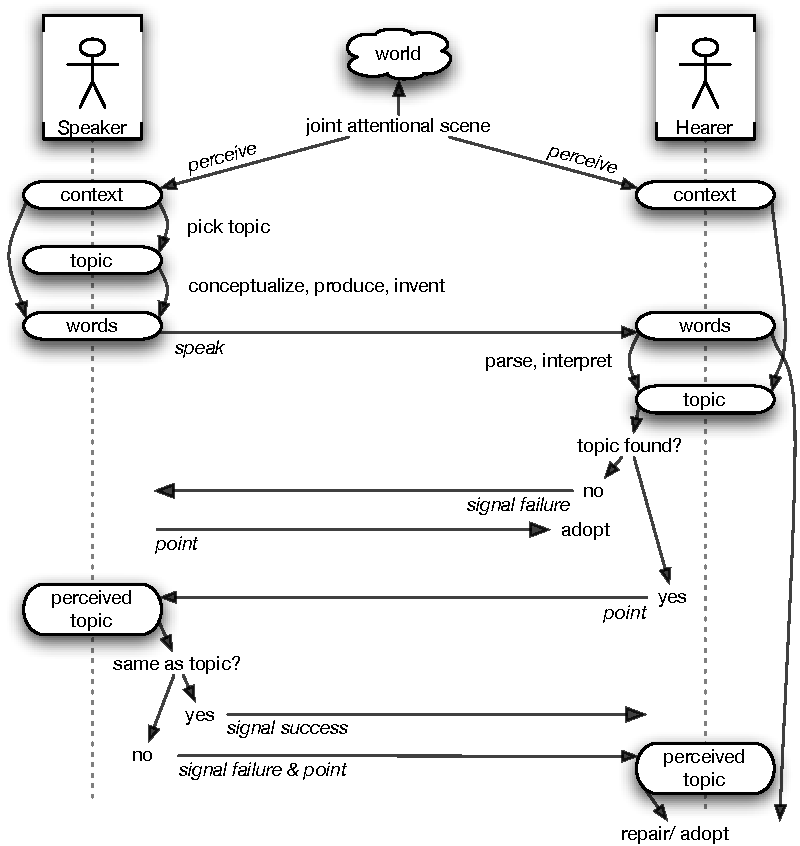
\includegraphics[width=0.80\textwidth]{figures/guessing-game-flow}}
  \caption{Main steps and mechanisms involved in a communicative
    interaction (see also Figure
    \ref{f:guessing-game-flow}).}
  \label{f:guessing-game-flow-2}
\end{figure}

At the begin of an experimental run, the population $P :=
\{a_1,a_2,\dots\}$ is created (we will by default use a population
size $|P| = 10$) and the agents $a_i \in P$ are initialized with empty
linguistic (and conceptual) inventories. Before each communicative
interaction, two agents are randomly drawn from this population and
assigned the communicative roles of speaker and hearer. To play a
language game, the speaker and hearer follow a built-in script that is
shown again in Figure \ref{f:guessing-game-flow-2} (see also Section
\ref{s:language-game}, page \pageref{s:language-game}). 

This particular type of language game will form the basis of all
experiments in this thesis and the particular lexicon formation models
will only differ in their strategies for representing, processing and
learning of lexicons and ontologies. We will now define these
mechanisms for the Naming Game and later on only discuss the
differences to this model:

\inparagraph{Lexicon representation} Each agent $a$ in the
population $P := \{a_1,a_2,\dots\}$ maintains a lexicon $L(a) :=
w_1(a),w_2(a),\dots$ consisting of a set of words $w(a)$. A word is
represented as a three tuple $w := \langle m(w), f(w), \gamma(w)
\rangle \in {\cal M}\times{\cal F}\times \mathbb{R}$, which is an
association of a meaning $m(w) \in {\cal M}$ to a form $f(w) \in {\cal
  F}$ with an association weight $\gamma(w)$ representing the agent's
confidence in that association. ${\cal M}$ is the set of possible word
meanings, ${\cal F}$ the set of possible word forms and $\gamma(w)$ a
real value with $0 \leq \gamma(w) \leq 1$.

\inparagraph{Perception} The world in which the agents interact
consists of shared atomic meanings $m \in {\cal M}$, which can be
anything but are typically seen as `individual objects'. In each
interaction both the speaker and hearer are provided with the vector
of all meanings in the world as their perception of the scene. By
default, the number of meanings in the world $|{\cal M}|$ is 10 and
thus, the context for each agent always consists of 10 `objects':
\begin{verbatim}
(obj-1 obj-2 obj-3 obj-4 obj-5 obj-6 obj-7 obj-8 obj-9 obj-10)
\end{verbatim}

\inparagraph{Topic selection} The speaker randomly selects one of the
objects in the context as the topic of the interaction.

\inparagraph{Conceptualization} In the Naming Game, the world already
provides pre-conceptualized meanings and consequently, the meaning
chosen as the topic is the meaning $m$ to be expressed.

\inparagraph{Production} The speaker looks up his lexicon for all
words that have $m$ as their meaning and from these selects the word
with the highest association score. When multiple words for meaning
$m$ have the highest score, a random choice is made.

\inparagraph{Invention} When the lexicon does not contain a word for
meaning $m$, then a new word $w=\langle m, f, \gamma_{i}\rangle$ with
a new unique form $f$ and an initial word score $\gamma_i$ of 0.5 is
created and stored in the lexicon of the agent. The new form $f$ is
guaranteed to be unique during an experimental run (no word form is
invented twice) and typically consists of three random consonant-vowel
combinations (e.g. ``fuzobi'' or ``kalige''). After invention,
production is repeated with the updated lexicon.

\inparagraph{Utterance} The single form produced by the speaker,
possibly after invention, is sent as the utterance to the hearer.

\inparagraph{Parsing} The hearer looks up his lexicon for the word
that matches the utterance (with no possibility of associating multiple
meanings to a form, there is always only one or no such word). The
meaning of that word is the meaning parsed by the hearer.

\inparagraph{Interpretation} In the Naming Game, the parsed meaning is
immediately treated as the topic understood by the hearer, no further
semantic interpretation is necessary.

\inparagraph{Pointing, communicative success and feedback} When the
hearer is able to parse the utterance and to interpret a topic, he
points to the topic by sending the meaning such as \texttt{obj-7} to
the speaker. The speaker compares the received meaning with his own
intended topic and signals a communicative success when this is the
case and a communicative failure otherwise. When the hearer does not
know the word uttered, he immediately signals a communicative failure
and the speaker then points to the intended topic.

\inparagraph{Adoption} Both when the hearer does not know a word form
$f$ or when he pointed to the wrong topic (which does not happen in
the Naming Game), the speaker will point to the intended topic
$m$. The hearer then adopts the new convention by storing a new word
$w=\langle m, f, \gamma_{i}=0.5\rangle$ in his own lexicon.

\inparagraph{Consolidation} Based on the outcome of the game, the
speaker and hearer update their lexicons in order to be more
successful in future interactions. When the interaction failed, then
both agents update the score of the word used in production
respectively in parsing by the value $\Delta_f = -0.1$. Words with a
score of 0 or smaller are removed from the lexicon. In the case of
communicative success, the scores of the words used are updated by
$\Delta_s = 0.1$ (and set to 1.0 if the result is greater) and the
scores of all words in the lexicon that have the same form are updated
by $\Delta_i = 0.1$ (\emph{lateral inhibition}, again, words with a
score of 0 or below are removed from the lexicon).


\section{Alignment dynamics}


\begin{figure}[t]
  
\renewcommand{\arraystretch}{1.3}{
\begin{tabular}{@{}llp{1cm}llp{1cm}l@{}}
  \# & speaker & topic speaker & utterance & hearer & topic hearer & success? \\
  \hline
100 & agent 5 & \texttt{obj-3} & \textit{``bukopa''} & agent 9 & \texttt{obj-3} & yes \\
101 & agent 3 & \texttt{obj-3} & \textit{``wosogi''} & agent 7 & \texttt{} & no \\
102 & agent 6 & \texttt{obj-7} & \textit{``tevaso''} & agent 2 & \texttt{} & no \\
103 & agent 9 & \texttt{obj-8} & \textit{``razitu''} & agent 4 & \texttt{} & no \\
104 & agent 6 & \texttt{obj-5} & \textit{``salusu''} & agent 8 & \texttt{obj-5} & yes \\
105 & agent 2 & \texttt{obj-3} & \textit{``xiliza''} & agent 7 & \texttt{obj-3} & yes \\
106 & agent 7 & \texttt{obj-1} & \textit{``ligita''} & agent 8 & \texttt{} & no \\
107 & agent 9 & \texttt{obj-9} & \textit{``navino''} & agent 3 & \texttt{obj-9} & yes \\
108 & agent 5 & \texttt{obj-10} & \textit{``pinobe''} & agent 8 & \texttt{} & no \\
109 & agent 1 & \texttt{obj-10} & \textit{``sifubi''} & agent 3 & \texttt{} & no \\
110 & agent 10 & \texttt{obj-6} & \textit{``kiduze''} & agent 6 & \texttt{obj-6} & yes \\
111 & agent 5 & \texttt{obj-10} & \textit{``pinobe''} & agent 1 & \texttt{} & no \\
112 & agent 10 & \texttt{obj-7} & \textit{``dezosa''} & agent 6 & \texttt{} & no \\
113 & agent 1 & \texttt{obj-1} & \textit{``sewapa''} & agent 7 & \texttt{} & no \\
114 & agent 10 & \texttt{obj-7} & \textit{``dezosa''} & agent 3 & \texttt{} & no \\
\end{tabular}}


%%% Local Variables: 
%%% mode: latex
%%% TeX-master: "../phdbook"
%%% End: 

  \caption{Overview of 15 consecutive interactions from game 100
    on. It shows the agents that are interacting, the topic chosen by
    the speaker, the utterance formed, the topic understood by the
    hearer (when successfully parsed) and whether the agents reached
    communicative success.}
  \label{f:ng-trace}
\end{figure}

With all these mechanisms in place, the population is able to
successfully create and align a shared lexicon for the meanings in the
world through series of such languages games. Figure \ref{f:ng-trace}
shows an example of 15 consecutive interactions from game 100
on. Within these early stages of the alignment process, most
interactions fail, although in some of them words are used that both
the speaker and hearer know. Interaction 100 was played between agent
5 and agent 9 and the speaker picks \texttt{obj-3} as the topic of the
conversation. The word chosen by the speaker is ``bukopa'', which in
turn is successfully interpreted by the hearer as \texttt{obj-3},
eventually making the interaction a success. In contrast, interaction
101 is an example of a failed game. The speaker agent 3 utters
``wosogi'' for the meaning \texttt{obj-3}, which the hearer agent 7
does not know yet. Note that in the Naming Game, an interaction is
immediately a success when the hearer knows the word, because agents
directly perceive the meanings from the world and thus never associate
a `wrong' meaning to a form in adoption.



\begin{figure}[t]
  \begin{tabular}{cp{1cm}c}
    interaction 250 & & interaction 2500 \\
    & & \\
    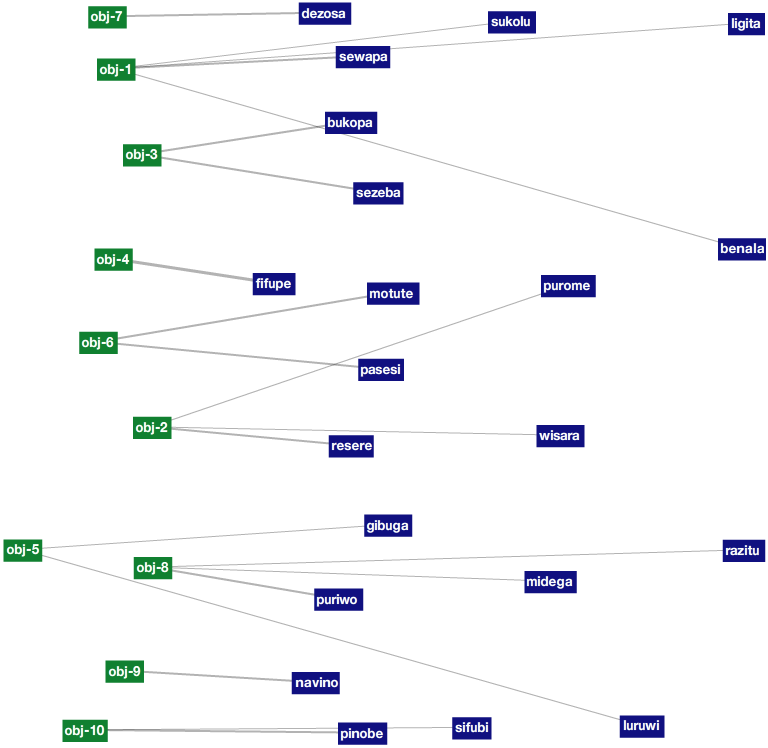
\includegraphics[scale=0.4]{figures/ng-lexicon-250} & &
    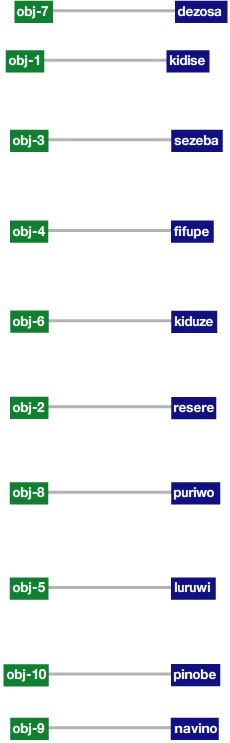
\includegraphics[scale=0.4]{figures/ng-lexicon-2500} \\
    & & \\
  \end{tabular}
  \caption{Network representation of the complete lexicon of the first
    agent in the population after 250 interactions (left) and 2500
    interactions (right). In each network, word meanings are drawn on
    the left and forms on the right. Each line represents a word in
    the lexicon of the agent, the line widths denote the strength of
    the association.}
  \label{f:ng-lexicon}
\end{figure}


Furthermore, even within these few games the population uses three
different forms for \texttt{obj-3}. This is because speakers
independently invent words for new meanings and hearers adopt words
from different speakers for the same meanings. To illustrate this,
Figure \ref{f:ng-lexicon} shows the lexicon of agent 1 after game 250
and after game 2500. After interaction 250, the agent associates up to
five different word forms to each of the meanings, which get reduced
to one per meaning after 2500 interactions. 

\startfiguregroup

\begin{figure}[t]
  
{\renewcommand{\arraystretch}{1.5}
\begin{tabular}{@{}p{1.2cm}|p{1.6cm}@{}p{0.8cm}@{}|p{1.6cm}@{}p{0.8cm}@{}|p{1.6cm}@{}p{0.8cm}@{}|p{1.6cm}@{}p{0.8cm}@{}}
meaning & agent 1 &  & agent 2 &  & agent 3 &  & agent 4 & \\
\hline
\texttt{obj-1}&\textit{``zasala''}


\textit{``milozo''}
&0.50

0.30&\textit{``milozo''}


\textit{``zasala''}
&0.50

0.50&\textit{``botewi''}


\textit{``zasala''}


\textit{``milozo''}


\textit{``legubu''}
&0.50

0.50

0.30

0.30&\textit{``zasala''}


\textit{``botewi''}
&0.30

0.50\\
\hline
\texttt{obj-2}&\textit{``zaxiwu''}
&0.80&\textit{``zaxiwu''}
&0.60&\textit{``dovege''}
&0.40&&\\
\hline
\texttt{obj-3}&\textit{``gokaso''}


\textit{``dotopi''}


\textit{``malixe''}
&0.40

0.40

0.40&\textit{``malixe''}


\textit{``dotopi''}


\textit{``fivine''}
&0.50

0.40

0.50&\textit{``dotopi''}


\textit{``nobaxo''}


\textit{``fivine''}
&0.50

0.40

0.50&\textit{``dotopi''}
&0.30
\end{tabular}}


  \caption{Forms associated to three different meanings by the first
    four agents of a population of 10 after 250 interactions.}
  \label{f:ng-lexicon-250}
\end{figure}

\begin{figure}[t]
  
{\renewcommand{\arraystretch}{1.5}
\begin{tabular}{@{}p{1.2cm}|p{1.6cm}@{}p{0.8cm}@{}|p{1.6cm}@{}p{0.8cm}@{}|p{1.6cm}@{}p{0.8cm}@{}|p{1.6cm}@{}p{0.8cm}@{}}
meaning & agent 1 &  & agent 2 &  & agent 3 &  & agent 4 & \\
\hline
\texttt{obj-1}&\textit{``milozo''}
&1.00&\textit{``milozo''}
&1.00&\textit{``milozo''}
&1.00&\textit{``milozo''}
&1.00\\
\hline
\texttt{obj-2}&\textit{``zaxiwu''}
&1.00&\textit{``zaxiwu''}
&1.00&\textit{``zaxiwu''}
&1.00&\textit{``zaxiwu''}
&1.00\\
\hline
\texttt{obj-3}&\textit{``gokaso''}
&1.00&\textit{``gokaso''}
&1.00&\textit{``gokaso''}
&1.00&\textit{``gokaso''}
&1.00
\end{tabular}}

  \caption{Associations to three meanings after 2000 interactions.}
  \label{f:ng-lexicon-2000}
\end{figure}

\stopfiguregroup

From the perspective of the population, Figure \ref{f:ng-lexicon-250}
shows snapshots of the first four agents' lexicons for three different
meanings after 250 played games. Their lexicons show a very low
coherence, with the numbers of associations and their forms greatly
varying. Whereas all four agents at least already have adopted an
association with the same form for \texttt{obj-2} and \texttt{obj-3}
(``resere'' and ``fodato''), this is not the case for \texttt{obj-1}:
Of all the four forms associated by agent 1 to this meaning, only one
(``sewapa'') is shared with one other agent.

\begin{figure}[t]
  \gnuplotfigure{figures/ng-word-form-scores-obj-3}
  \caption{Evolution of words in the population for the meaning
    \texttt{obj-3}. Each line shows for a single form the
    corresponding word scores averaged over all agents that know the
    form.}
  \label{f:ng-word-form-scores-obj-3}
\end{figure}


\begin{figure}[t]
  \gnuplotfigure{figures/ng-word-form-scores-obj-3-agent-1}
  \caption{Scores for forms associated by the first agent to the
    meaning \texttt{obj-3}.}
  \label{f:ng-word-form-scores-obj-3-agent-1}
\end{figure}


However, due to the strategies of 1) updating word scores based on the
outcome of the game, of 2) laterally inhibiting competing
associations, and of 3) preferring words with higher scores, the
population quickly reaches coherence. Figure \ref{f:ng-lexicon-2000}
shows the lexicons of the same four agents after 2000
interactions. For each of the three meanings, the population agreed on
a single form with 1.0 as the association score. Which of the forms
from the early stages `survives' this selection process can not be
completely determined by looking at the lexicons in Figure
\ref{f:ng-lexicon-250}, but it is clear that associations which are
known to more agents and which have a higher average score in the
population are more likely to become conventionalized.

Figure \ref{f:ng-word-form-scores-obj-3} shows for each form connected
by the population to the meaning \texttt{obj-3} the average
association scores across all agents. The form that eventually wins
(``sezeba'') is created very early on and competes with the form
``bukopa'' for dominance until around interaction 1000, after which
``sezeba'' asserts itself and ``bukopa'' slowly starts loosing the
competition, before it gets eliminated at around interaction 1800. All
other four forms initially created by the population are quickly
lowered in score, and the last one (``wosogi'') is removed by the last
agent at round interaction 900. Nevertheless, individual agents might
undergo much different dynamics. Figure
\ref{f:ng-word-form-scores-obj-3-agent-1} shows the scores of words in
the lexicon of agent 1 for the meaning \texttt{obj-3}. This agent did
not have the winning form ``sezeba'' in his lexicon between
interactions 400 and 500, only after which he re-adopted it and used
it most of the time. Similarly, the already eliminated form ``bukopa''
gets adopted again after interaction 1000 and because agent 1
successfully uses the word one time in the role of the hearer (as
speaker he would have chosen the still higher-scored form ``sezeba''),
the previously more successful ``sezeba'' becomes reduced in score due
to lateral inhibition. 


\begin{figure}[t]
  \gnuplotfigure{figures/ng-word-scores}
  \caption{Evolution of the first agent's lexicon over 2500
    interactions. Each line represents the score of a single word as
    it changes over time.}
  \label{f:ng-word-scores}
\end{figure}

Furthermore, Figure \ref{f:ng-word-scores} shows the evolution of
association scores of all words in the lexicon of agent 1. Despite the
previous example (which is in fact rare), most words that reach a
certain score above the initial words score of 0.5 win the competition
over their competitors and all other words become quickly
removed. After around interaction 1200, the lexicon does not change
anymore and all conventionalized forms remain at a score of 1.\\


\begin{figure}[t]
  \gnuplotfigure{figures/ng-success+lexicon-size}
  \caption{Main dynamics of the Naming Game. Communicative success
    (measure \ref{m:communicative-success}, page
    \pageref{m:communicative-success}) and lexicon size (measure
    \ref{m:lexicon-size}) are averaged over 10 repeated series of 2500
    interactions.}
  \label{f:ng-success+lexicon-size}
\end{figure}

\begin{measure}[b]{Lexicon size}{m:lexicon-size}
  Measures the average number of words known by the population. The
  number of meaning-form associations in each agent's lexicon is
  counted and averaged over the number of agents:
  $$v = \frac{\sum_{i=1}^{|P|} |L(a_i)|}{|P|}$$
  Values $v$ are averaged over the last 250 interactions.
\end{measure}

Finally and most importantly, the alignment dynamics of the population
can be analyzed quantitatively. As already discussed in Section
\ref{s:evaluating-language-games} on page
\pageref{s:evaluating-language-games}, communicative success, i.e. the
fraction of interactions in which the speaker reached his
communicative goal, is our main criterion for evaluating the
performance of language game experiments. Figure
\ref{f:ng-success+lexicon-size} shows the evolution of this measure
over 2500 consecutive interactions: after 600 interactions, in 80\% of
the games communicative success is reached, and after about 1500
interactions, success reaches and remains at 100\%. A second crucial
measure is lexicon size, i.e. the average number of words in the
lexicon of each agent (also shown in Figure
\ref{f:ng-success+lexicon-size}). After an initial phase of invention
and adoption, at around interaction 300, each agent knows about 22
word forms. After that, word score update based on success and lateral
inhibition reduce the number of words, before it reaches 10 at around
interaction 1500. A lexicon size of 10 is considered to be `optimal',
because there are 10 different meanings in the world and an inventory
of 10 words for these meanings is the most cognitively efficient means
to communicate about these meanings in terms of processing and
ambiguities.


\begin{figure}[p]
  \gnuplotfigure{figures/ng-synonymy+coherence}
  \caption{Lexicon coherence (measure \ref{m:lexicon-coherence}),
    frequency of lexicon changes (measure
    \ref{m:frequency-of-lexicon-changes} and average number of forms
    per meaning (measure \ref{m:synonymy}) and averaged over 10
    repeated series of 2500 interactions.}
  \label{f:ng-synonymy+coherence}
\end{figure}


\begin{measure}[p]{Lexicon coherence between speaker and
    hearer}{m:lexicon-coherence}
  Provides a measure for how similar the lexicons of the interacting
  agents are. The degree of lexicon overlap between the speaker $s$
  and the hearer $h$ of the current interaction is computed as the
  fraction of form meaning associations that are shared by speaker and
  hearer and all words known by speaker and hearer:
  $$v=\frac{|L(s) \cap L(h)|}{|L(s)| + |L(h)|}$$
  Association weights of words are ignored when forming the
  intersection between the two lexicons. Values $v$ are averaged over
  the last 250 interactions.\\

  A slightly more precise measure for coherence in the population
  would be to compare the lexicons of all agents. But because
  computing coherence between all pairs of agents would be very
  costly, we chose to use coherence between speaker and hearer as a
  approximation for population coherence.
\end{measure}


\begin{measure}[p]{Frequency of lexicon changes}{m:frequency-of-lexicon-changes}
  Measures how stable the agents' lexicons are. For each interaction
  in which either the speaker or the hearer add or remove a word from
  their inventories, a value of 1 is recorded, for all others
  0. Values are averaged over the last 250 interactions.
\end{measure}


\begin{measure}[p]{Average number of forms per meaning (synonymy)}{m:synonymy}
  The average number of forms associated to each meaning by an agent
  is averaged over all agents in the population:
  $$v = \sum_{i=i}^{|P|}{\frac{|L(a_i)|}{|\{m:m \in {\cal M}\;\wedge\;\exists w ( w \in L(a_i) \wedge m_w(w) = m)  \}|}}\;/\;|P|$$
  Values $v$ are averaged over the last 250 interactions.
\end{measure}

Additionally, we will use measures of coherence, stability, and
ambiguities in inventories for evaluating the performance of language
games in this thesis (see Figure
\ref{f:ng-synonymy+coherence}). Lexicon coherence externally compares
the lexicons of speaker and hearer with respect to how similar they
are in terms of the fraction of shared form-meaning
associations. Coherence reaches 100\% soon after 1500 interactions,
but the curve slightly lags behind communicative success because even
when agents already consistently use the same forms for a particular
meaning, there are still varying competing forms that still need to be
eliminated by lateral inhibition (see also Figures
\ref{f:ng-word-form-scores-obj-3}-\ref{f:ng-word-scores}). 

Frequency of lexicon changes provides a measure for the stability of
the agents' lexicons by counting how often agents add or remove words
in their lexicons. At the beginning, speakers invent words or hearers
adopt words in almost every interaction, and after around interaction
500, when lateral inhibition results in a peak in the number of words
that are removed, the slope of stability increases. But similar to
coherence, complete stability is only reached much later than complete
communicative success (at around interaction 2000), because
lower-scored competing words still need to be removed from the
lexicons.

Finally, the average number of forms associated to each meaning is a
indicator for ambiguities in the agents' lexicons. This measure is
often also referred to as \emph{synonymy}, but the `synonyms' in the
lexicons of our agents are of a different quality than those found in
the real world: here there are competing forms for exactly the same
meaning, whereas in natural languages they are rather seen as words
with similar meanings, but still carrying semantic distinctions. In
the Naming Game, synonymy is directly correlated with lexicon size,
because the number of meanings to be expressed is fixed and there are
no word meaning ambiguities in adoption. The curves for lexicon size
and number of forms per meaning look exactly the same. When lexicon
size peaks at interaction 300 with 22 words, the degree of synonymy is
2.2, and at the optimal size of 10 words, there is only one form per
meaning.


\section{Other alignment strategies \& scaling}
\label{s:ng-alignment-strategies}

The main challenge for aligning lexicons in the Naming Game is the
elimination of competing word forms for the same meanings
(synonymy). The common strategy used for this is to update association
scores based on communicative success and to laterally inhibit
competing forms. However, other strategies are possible and in Figures
\ref{f:ng-alignment-strategy-vs-lexicon-size}-\ref{f:ng-alignment-strategy-vs-lexicon-changes}
we will compare four of them with the update dynamics discussed above
(in the graphs called ``update + lateral inhibition'').

\startfiguregroup

\begin{figure}[t]
  \gnuplotfigure{figures/ng-alignment-strategy-vs-lexicon-size}
  \caption{Compar\-ison of four different alignment strategies: lexicon
    size.}
  \label{f:ng-alignment-strategy-vs-lexicon-size}
\end{figure}

\begin{figure}[t]
  \gnuplotfigure{figures/ng-alignment-strategy-vs-communicative-success}
  \caption{Compar\-ison of four different alignment strategies:
    communicative success.}
  \label{f:ng-alignment-strategy-vs-communicative-success}
\end{figure}

\begin{figure}[t]
  \gnuplotfigure{figures/ng-alignment-strategy-vs-lexicon-changes}
  \caption{Compar\-ison of four different alignment strategies:
    frequency of lexicon changes.}
  \label{f:ng-alignment-strategy-vs-lexicon-changes}
\end{figure}

\stopfiguregroup

First, a strategy that we call ``no alignment'' does not change
association scores at all at the end of an interaction (the parameters
for word score in case of success $\Delta_s$, in case of failure
$\Delta_f$ and for lateral inhibition $\Delta_i$ are all set to
0). But still, although later than with the other strategies, the
population reaches almost complete communicative success after 2500
interactions. Nevertheless, average lexicon size increases to a stable
level of above 50, without ever decreasing again. Since all
associations remain at their initial word score of 0.5, speakers
essentially make a random choice when producing for a specific
meaning. What happens is that every form ever invented by a speaker
needs to be learnt by all other agents in the population in order to
reach success.

The second strategy ``update based on success'' only updates the
associations used by the speaker and hearer for producing and parsing
(and performs no lateral inhibition, $\Delta_s=0.1$, $\Delta_f=-0.1$,
$\Delta_i=0$). Communicative success is reached much faster than with
the default ``update + lateral inhibition'' strategy, but again
lexicon size does not reach the optimum of 10 but remains at a stable
plateau of about 33 words on average. This is because once a form wins
over its competitors, there is no chance for synonyms to be lowered in
score (which in this strategy is only possible through use in a failed
interaction). As a result, a number of `successful' forms for each
meaning will reach a score of 1.0 and speakers will randomly choose
from them, as with the previous strategy. All other associations will
not be used anymore, but remain in the lexicons of the agents.

These `unused' words can be eliminated with the third strategy
``update + constant decay''. In addition to updating scores of used
words based on the outcome of the game with $\Delta_s=0.1$,
$\Delta_f=-0.1$ and $\Delta_i=0$, the score of each association in the
lexicon is changed by a parameter $\Delta_d=-0.05$ divided by the
number of words in the lexicon. When words reach a score of 0 or
below, they are removed from the lexicon. This in a way creates
`blind' lateral inhibition dynamics, since words which are not
successfully used slowly become removed and only words who are
frequently used in successful interactions survive. However, there are
two problems with this strategy. First, the choice of parameter
$\Delta_d$ is very difficult. If it's too high, then words that are
well conventionalized but that happened not to be used often enough
can get accidentally removed. And if it's too low, then synonyms
become removed only very late. Second, this strategy only works when
the meanings expressed by the agents are equally distributed over
time: words for specialized meanings that occur less often are very
unlikely to survive with these dynamics.

Finally, a fourth strategy ``competitor elimination on first success''
again does not update word scores at all. Instead, on the first
occasion that a word is used successfully, all associations with
competing forms are immediately removed from an agent's lexicon (this
behavior can be emulated by choosing the parameters $\Delta_s=0$,
$\Delta_f=0$ and $\Delta_i=-0.5$). Surprisingly, agents reach complete
success and stability also with this strategy, although a bit later
than with the other ones. On the other hand, agents need to remember
less words (lexicon size peaks at about 16) and they don't need to
maintain word scores, which increases cognitive economy, especially
when scaling to larger population sizes.\\

\startfiguregroup

\begin{figure}[t]
  \gnuplotfigure{figures/ng-alignment-delta-inhibit-vs-communicative-success}
  \caption{The impact of different values for the word score update
    parameter $\Delta_i$ on communicative success.}
  \label{f:ng-alignment-delta-inhibit-vs-communicative-success}
\end{figure}

\begin{figure}[t]
  \gnuplotfigure{figures/ng-alignment-delta-inhibit-vs-lexicon-size}
  \label{f:ng-alignment-delta-inhibit-vs-lexicon-size}
  \caption{The impact of different values for the word score update
    parameter $\Delta_i$ on lexicon size.}
\end{figure}

\begin{figure}[t]
  \gnuplotfigure{figures/ng-alignment-delta-fail-vs-communicative-success}
  \label{f:ng-alignment-delta-fail-vs-communicative-success}
  \caption{The impact of different values for the word score update
    parameter $\Delta_f$ on communicative success.}
\end{figure}

\begin{figure}[t]
  \gnuplotfigure{figures/ng-alignment-delta-fail-vs-lexicon-size}
  \label{f:ng-alignment-delta-fail-vs-lexicon-size}
  \caption{The impact of different values for the word score update
    parameter $\Delta_f$ on lexicon size.}
\end{figure}

\begin{figure}[t]
  \gnuplotfigure{figures/ng-alignment-delta-success-vs-communicative-success}
  \label{f:ng-alignment-delta-success-vs-communicative-success}
  \caption{The impact of different values for the word score update
    parameter $\Delta_s$ on communicative success.}
\end{figure}

\stopfiguregroup

\noindent Other alignment strategies such as that the speaker always
imitates the last word heard for a meaning have been investigated by
\cite{kaplan05simple}, and he also found that the default strategy
``update + lateral inhibition'' is the best solution for dampening
competing forms for meanings in the Naming Game. Furthermore, this
strategy is very robust with respect to the actual parameters chosen
for updating word scores. In the literature, the values of
$\Delta_s=0.1$, $\Delta_f=-0.1$ and $\Delta_i=-0.2$ are often been
given some significance, but that choice is not crucial at all. As
shown in Figure
\ref{f:ng-alignment-delta-inhibit-vs-communicative-success}, almost
the same communicative success is reached for parameter $\Delta_i$ for
the whole range of values from 0 to 1. This parameter only affects how
soon agents remove synonyms from their lexicons, and as demonstrated
in Figure \ref{f:ng-alignment-delta-inhibit-vs-lexicon-size}, an
optimal lexicon size is reached quickly for the big range of values
$-1 \leq \Delta_i \leq -0.1$. 

Similarly, actual values for the score update parameter in the case of
communicative failure $\Delta_f$ have no real effect on communicative
success and lexicon size in the range of $-0.2\leq \Delta_i \leq 0$
(see Figures \ref{f:ng-alignment-delta-fail-vs-communicative-success}
and \ref{f:ng-alignment-delta-fail-vs-lexicon-size}). Only when
$\Delta_f$ is too high, then the alignment process has difficulties to
take off, because new words immediately get removed again from an
agent's lexicon on the first occasion that the word was used
unsuccessfully, which can easily happen with new conventions in a
population. Along the same lines, the choice of the association score
update parameter in case of success $\Delta_s$ is quite arbitrary. For
values $0.05 \leq \Delta_s \leq 1$ communicative success is more or
less the same (see Figure
\ref{f:ng-alignment-delta-success-vs-communicative-success}), only
when $\Delta_s$ is too small, negative updates from lateral inhibition
and on communicative failure do not get balanced anymore so that words
have more difficulties to reach high scores.\\

\startfiguregroup

\begin{figure}[t]
  \gnuplotfigure{figures/ng-population-size-vs-communicative-success}
  \label{f:ng-population-size-vs-communicative-success}
  \caption{Scaling of communicative success with increasing population
    size.}
\end{figure}

\begin{figure}[t]
  \gnuplotfigure{figures/ng-population-size-vs-lexicon-size}
  \label{f:ng-population-size-vs-lexicon-size}
  \caption{Scaling of lexicon size with increasing population size.}
\end{figure}

\stopfiguregroup

\noindent Finally, the Naming Game scales very well with increasing
population sizes, as demonstrated in Figures
\ref{f:ng-population-size-vs-communicative-success} and
\ref{f:ng-population-size-vs-lexicon-size}. To keep the curves
comparable, values are plotted along the x axis over the number of
games played by each agent instead of the overall number of
interactions as in the graphs before. For example, for a population of
500 agents to play 100 interactions per agent, $100 * 500 / 2 = 25000$
games need to be played, because two agents take part in every
interaction. The evolution of communicative success takes the form of
a s-curve for all population sizes. After an initial phase with low
success, in which a lot of new forms become invented, more and more
conventions assert themselves and the slope of the curve steepens,
before eventually a plateau of complete success is reached. The curve
for lexicon size looks identical for all population sizes, with
maximums naturally being higher for larger populations, because more
agents independently invent words for the same meanings.

We do not show graphs for scaling with increasing world complexity,
because the Naming Game scales linearly with the number of objects in
the world. With no ambiguity for the hearer in guessing what the
meaning of an unknown word is, the words for each meaning are
negotiated independently. Consequently, aligning words for 20 meanings
in the world takes double as long than for 10 meanings. This is also
the reason for why Naming Game dynamics are often investigated for a
single meaning -- additional meanings do not any complexity to the
model.\\


\noindent Much more is known about the dynamics of Naming Game-like
models of distributed conventionalization processes (in fact, the
Naming Game is by far the most investigated lexicon formation model),
but with lesser relevance for the experiments in our thesis, we will
not discuss these results in depth. There are proofs that the model
always convergences \citep{devylder06how,ke02complexity} (which is
reassuring to know for our work), and convergence times
\citep{kaplan05simple} and scaling laws \citep{baronchelli06sharp} are
well understood. Since it is somehow an unnatural assumption that in
large populations all agents communicate with and learn from each
other with equal probability, the impact of communication network
structures where some agents are more central than others has been
studied by \cite*{dallasta06nonequilibrium}. Furthermore, the
emergence of atomic conventions has been studied in stochastic
game-theoretic frameworks \citep{shoham97emergence}, with Markov
processes \citep{ke02complexity} and in connectionist neural networks
\citep{hutchins95how}. Finally, the impact of stochasticity in
perception, pointing, memory and utterance perception (i.e. there is a
probability of error in transmission) has been investigated by
\cite{steels98stochasticity}.






%%% Local Variables: 
%%% mode: latex
%%% TeX-master: "phd-thesis"
%%% End: 
